\documentclass[runningheads]{llncs}
\setcounter{tocdepth}{2}
\makeatletter
\renewcommand*\l@author[2]{}
\renewcommand*\l@title[2]{}
\makeatletter
%
\usepackage{listings}
\usepackage{float}
\usepackage{tikz}
\usepackage[T1]{fontenc}
% T1 fonts will be used to generate the final print and online PDFs,
% so please use T1 fonts in your manuscript whenever possible.
% Other font encondings may result in incorrect characters.
%
\usepackage{graphicx}
% Used for displaying a sample figure. If possible, figure files should
% be included in EPS format.
%
\usepackage{hyperref}
% If you use the hyperref package, please uncomment the following two lines
% to display URLs in blue roman font according to Springer's eBook style:
\usepackage{color}
\renewcommand\UrlFont{\color{blue}\rmfamily}
\urlstyle{rm}
%
\begin{document}
%
\title{Kinode: A General-Purpose Sovereign Cloud Computer (DRAFT, PRIVATE)}
%
\titlerunning{Kinode – DRAFT, PRIVATE}
%
\author{Benjamin McCormick and
Nicholas B Ludwig % \and
% Third Author\inst{3}\orcidID{2222--3333-4444-5555}
}
%
% \authorrunning{doria}
% First names are abbreviated in the running head.
% If there are more than two authors, 'et al.' is used.
%
\institute{ }
% \institute{Princeton University, Princeton NJ 08544, USA \and
% Springer Heidelberg, Tiergartenstr. 17, 69121 Heidelberg, Germany
% \email{lncs@springer.com}\\
% \url{http://www.springer.com/gp/computer-science/lncs} \and
% ABC Institute, Rupert-Karls-University Heidelberg, Heidelberg, Germany\\
% \email{\{abc,lncs\}@uni-heidelberg.de}}
%
\maketitle              % typeset the header of the contribution
%
\begin{abstract}
Kinode is a software platform designed to integrate all facets of modern crypto application development.
Its node-based cloud computing model bridges the impedance mismatch between onchain protocols and web services.
Users can run their own services at both the interface and backend level.
Corporations or other entities can provide services in a permissionless, protocolized manner.
Developers can write apps in any programming language that compiles to Wasm, then distribute them to sovereign users. %TODO: what exactly do you mean by sovereign in this context? Let's be as clear as possible

Kinode is a lot of things: an operating system, an onchain namespace/global messaging primitive, a utility token for governing and assigning value to that namespace, an onchain PKI (Public-Key Infrastructure), and a DAO that controls both onchain assets and continued development of the OS.
All of these aspects work in lockstep to solve the problems that have heretofore discouraged developers from embracing peer-to-peer computing.

% \keywords{Operating System \and Decentralized \and Cloud \and Wasm \and Cryptocurrency \and Public-Key Infrastructure \and Namespace \and Peer-to-Peer }
\end{abstract}
%
%
%
\tableofcontents
%
%
%
\section{Overview}
\label{sec:overview}

Cryptocurrency, specifically smart contract blockchains, have triggered a nascent revolution in permissionless protocols: software in which all can participate and none can can shut down.
But progress towards a fully decentralized, permissionless internet has stagnated even as specific niches like decentralized finance (DeFi) flourish.
We believe that this progress is constrained less by blockchain speed and throughput than by an underdeveloped offchain computing substrate.

Recall the singular problem blockchains are designed to solve: preventing the double-spending of a cryptographically-owned asset.
\footnote{link to bitcoin whitepaper perhaps and rephrase to match}
The mechanism to achieve this, now well-proven, expanded to turing-complete VMs, and replicated dozens of times, is simple: signed transactions validated by a decentralized validator set and deposited into an append-only distributed ledger.

But which operations \textit{actually} benefit from an onchain transaction?
Permissionless financial transactions obviously require blockchains, at least at the moment of settlement.
Similarly for operations that mutate ownership of an asset.
Smart contracts have proven that double-spend prevention can productively be applied to any digital asset that requires guaranteed global consensus on the order and provenance of operations.

Now, which operations \textit{do not} benefit from such guarantees?
For one, any action that only requires a single digital signature from a single entity. %TODO: do we need to explain WHY?
Blockchain transactions are similarly unnecessary for actions undertaken between trusted parties, which, in fact, comprise a large portion of online transactions.
It turns out that the category of networked operations that do not require global consensus is much larger than the category of those that do benefit from being blockchain transactions.

Some protocols, like many in DeFi, function perfectly fine with no user interaction outside their onchain transaction protocol.
The user interface for such a protocol is merely a wrapper over the smart contract deployed onchain.
There is a vast landscape of possible protocols, however, which do not fit entirely into the transaction paradigm.
Forcing these protocols into this model has led to countless failures. %TODO: not entirely clear what the "transaction paradigm" is here

Some believe that merely increasing transaction throughput by a few orders of magnitude can be a solution to this problem. %TODO: Same as above, I don't think "this problem" is clearly defined—the problem of using onchain transactions where they are not necessary?
We do not.
There are significant costs to placing transactions in a globally-distributed ledger—not only monetary, but also in terms of latency, data storage, and compute overhead.
Transactions will \textit{always} present an impedence mismatch and be an inferior technical solution for certain operations. %TODO: could use one elaborating phrase..."certain operations that..."
Until we provide a proper solution for such operations, ``Web3'' will simply never outcompete ``Web2''.

\begin{figure}[H]
    \centering
    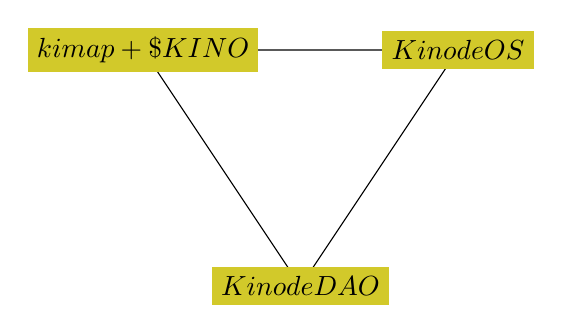
\begin{tikzpicture}
    \draw (0,3) node[fill=yellow!80!black]{$kimap+\$KINO$}
    -- (4,3) node[fill=yellow!80!black]{$Kinode OS$}
    -- (2,0) node[fill=yellow!80!black]{$Kinode DAO$}
    -- cycle;
    \end{tikzpicture}
    \caption{Architecture of Kinode.}
    \label{fig:triangle}
\end{figure}

The goal of the Kinode Hyperstructure
\footnote{description and link to hyperstructures}
is to present a permissionless substrate for computing.
Smart contract blockchains provide access to global consensus state for provenance over digital assets–Kinode does ``everything else''.
In this paper, we present an operating system, an onchain global namespace, a value assignment and ranking mechanism, and a governance structure for those components.

\section{Kimap}
\label{sec:kimap}

Historically, discoverability of both \textit{peers} and \textit{content} has been a major barrier for peer-to-peer developers.
Discoverability can present both social barriers (finding a new user on a game or chat) and technical obstacles (node software aquiring networking information for particular username).
Many solutions have been designed to address this problem, but so far, the ``devex'' (developer experience) of deploying centralized services has continued to outcompete the p2p discoverability options available.
Why is this?
\begin{enumerate}
    \item Libraries such as \verb|libp2p|, while effective at their goal of providing p2p primitives, do not provide the ``batteries included'' identity, discoverability, and network-effect-potential of more traditional centralized alternatives, and can also be difficult to approach for new developers.
    \item ``Pure'' peer-to-peer protocols still rely on hardcoded lists to bootstrap new entrants.
    \item Constructs such as distributed hash tables, frequently used in p2p protocols, are complex to properly implement.
\end{enumerate}
We believe that in order for decentralized software to outcompete, it must be both easier to reason about (for a developer) and more effective at delivering desirable user experiences.

These principles drive the design of kimap.
\begin{enumerate}
    \item All globally-shared data must be \textit{in one place}.
    This property ensures that a full, up-to-date snapshot data is easily read.
    \item For Kinode, that ``one place'' is onchain inside a single smart contract.
    \item All data necessary to bootstrap peer-to-peer interaction must be available within the globally-shared map.
    \item Any ``missing piece'' required to complete handshakes or source peers will result in unreliability and re-centralization.
\end{enumerate}

Kimap is an onchain key-value store inspired by \href{https://github.com/dapphub/dmap}{dmap}, a minimalist onchain path-formatted key-value store.
It serves as the base-level shared global state that all nodes use to share critical data to the entire network.
Like dmap, kimap is organized as a hierarchical path system and has mutable/immutable keys.
Several aspects of the map implementation are customized for the ``namespace'' use case.
However, the most important details that enable dmap to be read from and verified easily remain in place.

With this in mind, the following specification describes kimap:

\begin{enumerate}
    \item All keys are strings containing exclusively characters 0-9, a-z (lowercase), - (hyphen), and \_ (underscore) [TODO maybe not underscore? need to be compatible with existing app names though..].
    This property ensures that a full, up-to-date snapshot data can be read easily.
    \item An entry is a path made of ordered keys.
    \item Every entry has an owner address, which can be a contract or an EOA.
    \item The owner address can transfer the entry to a new owner and mint keys directly below the entry in the path hierarchy. For example, if a wallet owns \verb|mypath.network|, that wallet can mint \verb|hello.mypath.network|.
    \item Every kimap entry is an ERC-721 NFT (non-fungible token).
    Thus, each entry is a unique transferable onchain asset with a known ownership history.
\end{enumerate}

A key may be minted with the prefix \verb|~|. Such keys may not have keys minted beneath them: they are terminal nodes. The prefix denotes that such keys are used to store a bytes payload of readable data. %TODO: Byte payload? Byte's payload?
The format of the stored data is determined on a protocol-by-protocol basis depending on the key name. Any valid key name with the tilde-prefix may store data.

\begin{figure}[H]
    \centering
    \begin{lstlisting}
    os
        foo
            ~ip
            ~ws-port
            ~net-key
        bar
            ~routers
            ~net-key
    kino
        baz
            package
                ~metadata-hash
                ~metadata-uri
    eth
        alice
            ~routers
            ~net-key
        bob
            ~routers
            ~net-key
    \end{lstlisting}
    \caption{Example kimap.}
    \label{fig:example kimap}
\end{figure}

Fig.~\ref{fig:example kimap} shows an example with three top-level namespace entries, \verb|eth|, \verb|kino|, and \verb|os|.
Below those are a number of namespace entries that can be considered ``zones'', such as \verb|foo|, \verb|bar|, \verb|baz|.
The full path for \verb|foo|'s \verb|~ip| sub-entry would be \verb|~ip.foo.os|.
In this paper, we will sometimes use the term ``domain'' interchangeably with what we refer to here as a ``namespace entry''.
This is a useful shorthand, and in many ways, kimap does mirror the role of DNS in the worldwide web.
However, the ``domain'' analogy would be inaccurate if applied directly to all namespace entries because not all namespace entries participate in the KNS (Kinode Name System).
E.g., only entries containing \verb|~net-key| are used by the KNS protocol which runs \textit{on top} of the kimap.
Entries \verb|baz.kino| and \verb|package.baz.kino| have no sub-entries to describe their status as a domain in the KNS, and so the ``domain'' analogy breaks down for them.
The design of kimap is generic in the sense that many protocols are expected to share this global namespace for different purposes.
The specification of KNS itself, as a protocol operating on kimap, is described in Section~\ref{sec:kns}, as is the specification of the Kinode Package Manager, Section~\ref{sec:packagemanager}, which makes an appearance in this example.

\subsection{Top-Level Zones}
\label{sec:tld}

Entries at the top-level of kimap, with no parent entry, can be considered Top-Level Zones.

Minting of new TLZs in kimap is permissioned.
Top-level entries are valuable, because they produce new namespaces that can be applied to new protocols, entities, or individuals.
Allowing new TLZs to be created freely would lead to name-squatting and other perils clearly demonstrated by the history of similar namespaces. %TODO: such as? And what are the "other perils"
Instead, the distribution of TLZs over time is one of the key responsibilities of Kinode's governance apparatus, described in the Kinode DAO discussion in Section~\ref{sec:dao}.

Since every entry in the namespace can be owned by a contract, different control logic can be reliably implemented at the ownership level.
At first launch of kimap, a few selected TLZs will have ownership transferred to immutable contracts. %TODO: by the Kinode DAO?
Other TLZs will be time-locked in contracts, acting as a rent mechanism. %TODO: what do you mean by rent mechanism?

Why create a new namespace, given that others exist with established network effects?
Primarily, because Kinode OS needs it.
The goal of the OS is to create a fully-integrated programming environment, and existing namespace options are simply not designed to enable this.
This does not mean the namespace must operate in isolation–see the section on \hyperref[sec:extensibility]{extensibility} for a description of how other namespaces may be integrated with kimap.

\subsection{Namespace Hierarchy}
\label{sec:namespaces}

Each entry in kimap has write access to all of its sub-entries, at any level of nesting.
Even if \verb|package.baz.kino| is minted and transferred to different owner than \verb|baz.kino|, which itself is owned by a different address than \verb|kino|, the owner of \verb|kino| may transfer or edit data stored at \verb|~metadata-hash.package.baz.kino|.
There are two ways for the owner of a non-top-level entry to ensure control over their namespace entry: parent entries can be owned by an inert address (\verb|0x00..00|, e.g.) or owned by a contract which is programmatically incapable of mutating their entry.%TODO: how can the owner of a non-top level entry ensure that if they don't have the parent entry? Does that make most name spaces unsafe to own?

This property enables arbitrarily complex logic governing sub-namespaces of kimap.
A given namespace can be owned by a contract which implements rent logic, requiring regular payments for control over a sub-entry.
Or, an owner contract could dynamically re-allocate sub-entries as temporary or permanent rewards for auctions, gameplay, or other onchain activities.
We anticipate and welcome these experimental outcomes.

As part of Kinode DAO's responsibilities in guaranteeing the utility and reliability of the protocol, certain namespaces will be given over to immutable contracts at launch.
The \verb|os| TLZ, for example, will be controlled by a contract that allows any sub-entry to be minted freely, by anyone, and owned forever.
To prevent name squatting and generally dilute the value of this ``namespace of last resort'', minted sub-entries are required to be 9 or more characters long.
This also serves as a good example of the kind of custom logic a namespace may implement.

\subsection{Storing Data At Terminal Nodes}
\label{sec:terminalnodes}

At any level below the top in the kimap path hierarchy, a new key may be minted with the \verb|~| (tilde) prefix to signify that it stores a value.

Entries of this variety \textbf{may not} mint sub-entries, hence the prefix: one can use \verb|~my-data.hello.os| to store data while minting \verb|my-data.hello.os| in order to mint sub-entries beneath it, should one desire to do so.

Data is stored as bytes inside the contract map.
The owner of a namespace entry is the only address that can modify the data stored at that entry.
The interpretation of stored bytes is the responsibility of the protocol reading and writing from that entry.
Data can be mutable or immutable.
All data is public.
Protocols that wish to operate on private data may store hashes at namespace entries, or alternatively operate within the end-to-end encrypted Kinode networking protocol.

\subsection{Token-Bound Accounts}
\label{sec:tokenboundaccounts}

Each namespace entry that does not store data, i.e. does not have a \verb|~| prefix, is an ERC-6551\footnote{A standard which allows ERC-721 NFTs to have an attached Ethereum account:  https://eips.ethereum.org/EIPS/eip-6551} token-bound account.
This means that namespace entries are automatically endowed with a wallet, controlled by their owner, for receiving, holding, and sending digital assets that live on the same chain as kimap.
The address of each entry's token-bound account is deterministic based on the path value.
Thus, before a path is even minted, one can send assets to its future wallet address or otherwise operate on it.

Token-bound accounts are self-evidently useful but become particularly powerful when combined with the KNS protocol to give every node identity an attached wallet.

\subsubsection{Creation and Use}

A token-bound account is created automatically for every non-tilde-prefixed kimap entry.
The address of the account is deterministically generated based on the full path of the entry.
The owner of the entry has the ability to operate the account.

%TODO add more here

\subsection{Extensibility}
\label{sec:extensibility}

Kimap is designed to be generic and extensible.
Protocols such as KNS and the Kinode Package Manager extend kimap by interpreting the data stored at certain keys in a particular way.
A specific description of how this works can be seen in Section~\ref{sec:kns} and Section~\ref{sec:packagemanager}, respectively.

In the general case, a protocol specifies itself on kimap by declaring a set of \verb|~|-prefixed keys which are interpreted a certain way and endow certain properties to their parent key.
For example, a motd (``message of the day'') protocol might specify that the bytes stored at any \verb|~motd| key will be interpreted as a UTF-8 motd string for the parent key, which could be a node identity in the KNS.
If the owner of the key \verb|howdy.kino| wishes to participate in this protocol, it simply mints the key \verb|~motd.howdy.kino| and stores bytes there, perhaps \verb|[68 65 6c 6c 6f 20 77 6f 72 6c 64]|.


Extension of kimap is permissionless: any protocol can operate on the keys and data stored in the map.
Note that if two protocols use the same entry or entries to store data, key owners may be forced to choose between participating in one protocol or the other.
If an entry label is already in use by a popular protocol, developers creating a new protocol would be advised to either match the data format in current use for that entry label, or ensure non-overlap by prefixing/postfixing the entry label with a custom value.
For example, if the key \verb|howdy.kino| is the entry-of-interest, and the motd protocol described above is in common use, a different protocol that wishes to use the \verb|~motd| entry label could specify that it instead reads that label from \verb|~my-protocol-motd.howdy.kino|.

Another strategy for avoiding conflicts is to subdivide the namespace by storing a protocol's data entries at a nested path beneath the relevant entry.
If the key \verb|howdy.kino| is the entry-of-interest, and the motd protocol described above is in common use, a different protocol that wishes to use the \verb|~motd| entry label could specify that it reads that label from \verb|~motd.my-protocol.howdy.kino| rather than directly below.

\section{KNS, Kinode Name System}
\label{sec:kns}

Kinode Name System (KNS) is a protocol built on top of kimap (kimap is covered above in Section~\ref{sec:kimap}).
KNS transforms an entry in the kimap namespace into a \textit{node identity} for use in the Kinode network, where a ``node'' is an instance of Kinode OS, able to communicate p2p with other such nodes (see Section~\ref{sec:os} for more details).
Node identities are central to the programming model of Kinode OS.
Usually manipulated as strings in a process, a node's identity is the first component of an \verb|address|, which uniquely identifies a specific process, part of a package, published by a (different) \verb|node_id|, running on that particular node (see Section~\ref{sec:os} for definitions and discussion).

\subsection{Specification}
\label{sec:knsspec}

The definition of a node identity in the KNS protocol is any kimap entry that has a \verb|~net-key| sub-entry and either:
\begin{enumerate}
\item A \verb|~routers| sub-entry OR
\item An \verb|~ip| sub-entry AND at least one of:
	\begin{enumerate}
	\item \verb|~tcp-port| sub-entry
	\item \verb|~udp-port| sub-entry
	\item \verb|~ws-port| sub-entry
	\item \verb|~wt-port| sub-entry
	\end{enumerate}
\end{enumerate}

A sample of this protocol can be seen in Fig.~\ref{fig:example kimap}.
Two classes of nodes are defined: \textit{direct} and \textit{indirect}.
Direct nodes are those that publish an \verb|~ip| and one or more of the \verb|port| sub-entries.
Indirect nodes are those that publish \verb|~routers|. %TODO: this is the first time direct/indirect nodes have been mentioned. Perhaps worth linking to further discussion since it's relevant to how to think about the system byond what's described here

The data stored at \verb|~net-key| must be 32 bytes corresponding to an Ed25519 public key.
This is a node's signing key which is used across a variety of domains to verify ownership, including in the end-to-end encrypted networking protocol between nodes.
The owner of a namespace entry/node identity may rotate this key at any time by posting a transaction to kimap mutating the data stored at \verb|~net-key|.

The bytes at a \verb|~routers| entry must parse [TODO what encoding?] to an array of strings.
These strings should be node identities.
Each node in the array is treated by other participants in the networking protocol as a router for the parent entry.
Routers should themselves be direct nodes.
If a string in the array is not a valid node identity, or it is a valid node identity but not a direct one, that router will not be used by the networking protocol.
Further discussion of the networking protocol specification is presented in the Section~\ref{sec:osnetworking}.

The bytes at an \verb|~ip| entry must be 16 bytes corresponding [TODO clarify little or big endian] to a 128-bit unsigned integer.
This integer is translated to an IPv4 address if it is <32-bit.
Otherwise it is translated to an IPv6 address. [TODO clarify translation process]

Lastly, the bytes at any of the following port entries must be 2 bytes corresponding to a 16-bit unsigned integer: [TODO clarify little or big endian]

\begin{enumerate}
\item \verb|~tcp-port| sub-entry
\item \verb|~udp-port| sub-entry
\item \verb|~ws-port| sub-entry
\item \verb|~wt-port| sub-entry
\end{enumerate}
This integer is translated to a port number.
In practice, port numbers used are between 9000 and 65535.
Ports between 8000-8999 are usually saved for HTTP server use.

\subsection{Indexing}
\label{sec:knsindexing}

Events emitted by kimap are used to index map data.
Kinode OS provides all the primitives required to index effectively.

TODO more here: include the event data types and what values are indexed such that they can be used as filters.

\subsection{Adding Other Onchain Identity Primitives}
\label{sec:knsotherprimitives}

The KNS is not an attempt at replacing or competing with existing onchain identity primitives such as ENS and Lens.
Rather, it is designed to satisfy the public key infrastructure needs of the Kinode network.
It is of paramount importance that nodes can initiate secure communication with one another without the use of any data-set other than what is available publicly onchain.
Peer-discovery middlemen induce centralization and complicate networking protocols.

The structure of kimap means that KNS not only avoids competition with other identity primitives, but also seamlessly integrates them.
As of this paper, this has already been done for ENS protocol.
Here is a brief description of the procedure to do so:
\begin{enumerate}
    \item Create a contract to allow owners, and only owners, of a given identity primitive to mint their corresponding name in a kimap namespace controlled by this contract.
    \item Mint and transfer the top-level namespace entry corresponding to an outside identity primitive, \verb|lens| for example.
    \item If necessary, configure a LayerZero, or other such cross-chain messaging protocol, to allow owners of an identity primitive on another chain to verify their ownership on the chain that kimap is deployed on.
    \item The final result is that the owner of, for example, \verb|myname.lens| can now register \verb|myname.lens| in kimap and use it as their PKI entry for Kinode.
\end{enumerate}

\section{Kinode OS}
\label{sec:os}

This section discusses the architecture of Kinode OS.
For a more ``hands-on'' description of the OS, including detailed programming examples and documentation, go to \href{https://book.kinode.org/}{book.kinode.org}.

Kinode OS is a process virtual machine run to operate a ``node'' on the Kinode network.
At its core, the virtual machine wraps around a Wasm runtime
\footnote{Wasm is specified at https://webassembly.github.io/spec. Kinode uses Wasm for processes because it is a highly performant, language independent, portable, and sandboxable compilation target.}
which executes all userspace code.
After a node identity is registered onchain in the KNS, the operator should boot the OS using the private key matching the public \verb|~net-key| posted in the kimap.
Once this has been done, if the networking details (routers, IP, etc) are properly read from the kimap and matched by the runtime, that node is now ``online''.
Other nodes can interact with the booted node through the Kinode networking protocol by reading its KNS node identity and using the data stored there.

Kinode DAO develops and distributes Kinode OS.
Kinode DAO is currently developing a formal specification of all aspects of the virtual machine.
The runtime is as simple as possible, with a maximal amount of logic ejected to userspace and the rest stored in modules.
In the future, Kinode will benefit from ``client diversity'' as does a traditional blockchain: many implementations of the virtual machine
\footnote{The Wasm runtime is by a wide margin the most complex aspect of the OS, and at least a dozen such runtimes exist today, written in multiple languages.
This bodes well for future Kinode client diversity.}
will make the network more resistant to potential bugs and decentralize the development process, leading to productive ossification of core features, stability, and long-term strength.

While all packaged into a single executable, the OS can productively be described in 3 parts: a \textit{runtime}, a set of \textit{runtime modules}, and \textit{userspace}.
The ``kernel'' frequently referred to in this paper is in fact just a runtime module.

The runtime is a ``native'' (to whatever architecture it targets, which may be Unix, a browser, hardware...) program that manages node booting (including onchain registration) and (generally asynchronously or in parallel) executes the runtime modules.
Runtime modules are blocks of code written at the same level of abstraction as the runtime itself, but designed to resemble userspace processes.
These modules are registered in the kernel \textit{as} processes, meaning that they can be messaged by userspace in the system-wide request-response protocol and secured via capabilities.
Finally, userspace is comprised of all non-runtime-module processes executed virtually by the kernel.
These processes are always compiled to Wasm and comport to the Wasm Component Model\footnote{https://component-model.bytecodealliance.org/}.
They are adapted to the Kinode WIT file which defines the common interface that all processes must implement and provides a set of ``system calls'' afforded to userspace processes by the kernel.

The reference implementation built and maintained by the DAO is currently written in Rust, as are all the runtime modules.
It also comes with a number of pre-installed userspace packages that perform critical tasks.
In the future, other entities will likely seek to distribute their own implementations which may contain different pre-installed packages or even different runtime modules.

\begin{figure}
    \centering
    \begin{lstlisting}
    eth:distro:sys
    http_client:distro:sys
    http_server:distro:sys
    kernel:distro:sys
    kv:distro:sys
    net:distro:sys
    state:distro:sys
    terminal:distro:sys
    timer:distro:sys
    sqlite:distro:sys
    vfs:distro:sys
    \end{lstlisting}
    \caption{The full list of runtime modules in the OS distribution maintained by Kinode DAO as of this writing.}
    \label{fig:runtime modules list}
\end{figure}

\subsection{WIT}
\label{sec:oswit}

Wasm Interface Type\footnote{https://component-model.bytecodealliance.org/design/wit.html}, or WIT, is a format to describe types and function definitions which can be used in a Wasm component.
Kinode OS uses a single WIT file to define the types shared across all processes and provide a number of functions.
The functions fall into three categories:
\begin{enumerate}
    \item Self-configuration
    \item Capabilities management
    \item Message I/O
\end{enumerate}

WIT files are organized into worlds. All types and functions provided to Kinode processes are currently stored in one world labeled \verb|lib|.

\subsubsection{WIT Types}
\label{sec:oswittypes}

Discussion of the types presented here will occur throughout the rest of the OS description.
Some types in kinode.wit are omitted for brevity or because they are discussed later.

\begin{figure}[H]
    \centering
    \begin{lstlisting}
    record process-id {
        process-name: string,
        package-name: string,
        publisher-node: node-id,
    }
    record address {
        node: node-id,
        process: process-id,
    }
    record lazy-load-blob {
        mime: option<string>,
        bytes: list<u8>,
    }
    \end{lstlisting}
    \caption{Basic types in kinode.wit}
    \label{fig:WIT Types 1}
\end{figure}

An \verb|address| globally identifies a process running on a particular node.

A \verb|process-id| identifies a particular process by its publisher, package name, and process name.

\subsubsection{WIT Host Functions}
\label{sec:oswitfuncs}

WIT host functions must be implemented by the kernel.
The Wasm Component model allows these functions to be called by processes.

\begin{figure}[H]
    \centering
    \begin{lstlisting}
    // self-configuration
    print-to-terminal()
    set-on-exit()
    get-on-exit()
    get-state()
    set-state()
    clear-state()
    spawn()

    // capabilities management
    save-capabilities()
    drop-capabilities()
    our-capabilities()

    // message I/O
    receive()
    get-blob()
    send-request()
    send-requests()
    send-response()
    send-and-await-response()
    \end{lstlisting}
    \caption{Host functions in kinode.wit}
    \label{fig:WIT Functions}
\end{figure}

\subsubsection{WIT Process Format}
\label{sec:oswitprocess}

The process format enforced by kinode.wit is remarkably simple: it imports the types and functions defined in the main library world, and requires processes to implement a single function: \verb|init|.
\footnote{This does not preclude processes from implementing other functions.}

\begin{figure}[H]
    \centering
    \begin{lstlisting}
    world process {
        include lib;
        export init: func(our: string);
    }
    \end{lstlisting}
    \caption{Process world in kinode.wit}
    \label{fig:Process world}
\end{figure}

\verb|init| serves as the entry point for a process.
The kernel begins execution of a process by calling \verb|init|.
When \verb|init| returns, the process will cease execution.
\footnote{All processes are single-threaded. To perform parallel computation, one can spawn child processes.}

\subsection{Microkernel}
\label{sec:osmicrokernel}

Every aspect of the operating system, including the kernel itself, comports to a set of messaging rules defined by the microkernel\footnote{https://wiki.osdev.org/Microkernel} which is responsible for five things:
\begin{enumerate}
    \item Using a Wasm runtime
    \footnote{The reference implementation currently uses \href{https://wasmtime.dev}{Wasmtime}.}
    to execute compiled processes which implement the Kinode WIT standard, where execution includes managing their memory usage.
    \item Implementing the host functions, exposed to all processes, defined in Kinode WIT standard.
    \item Implementing the kernel API that allows processes with kernel-messaging capabilities to perform aspects of process management.
    \item Passing messages between all processes including to/from the kernel itself.
    \item Enforcing messaging capabilities.
\end{enumerate}

Messaging capabilities are a subset of the capabilities security model defined by the OS, issued by the kernel process, \verb|kernel:distro:sys|.
Each process can mark itself as either \verb|public| or \verb|private| at instantiation.
Public processes can be messaged by any other process.
Private processes, as enforced by the kernel, require that the message source holds their messaging capability.
See the discussion of capabilities in Section~\ref{sec:oscapabilities} for details on their use and how capabilities apply to processes running a remote node.

As of this writing, the kernel runtime module in Kinode DAO's implementation of the OS fits into about 2,700 lines of Rust.

\subsection{Message Passing}
\label{sec:osmessagepassing}

A message between two Kinode processes is either a request or a response.
A message has a single source \verb|address| and a single target \verb|address|.

\begin{figure}[H]
    \centering
    \begin{lstlisting}
    record request {
        inherit: bool,
        expects-response: option<u64>,
        body: list<u8>,
        metadata: option<json>,
        capabilities: list<capability>,
    }
    record response {
        inherit: bool,
        body: list<u8>,
        metadata: option<json>,
        capabilities: list<capability>,
    }
    variant message {
        request(request),
        response(tuple<response, option<context>>),
    }
    \end{lstlisting}
    \caption{Message type in kinode.wit}
    \label{fig:WIT Types 2}
\end{figure}

Messages are produced and consumed by Kinode processes.

If the node identity indicated in the target \verb|address| matches that of the local kernel or is simply the string \verb|our|, the message is routed directly through the kernel to the target (assuming the source has the capability to message the target or the target is public).
Otherwise, the message is routed through the networking runtime module, \verb|net:distro:sys| to the remote node indicated.

Ordering of messages between a given source and a given target is enforced by both kernel and networking protocol.
Messages are not otherwise ordered, meaning that if process A sends messages 1, 2, 3 to process B, and process B sends messages 4, 5, 6 to A, no guarantees are enforced other than that process B will receive messages 1, 2, 3 in that order and process A will receive 4, 5, 6 in that order.
If process C sends message 7 to A, it may be received before 1, after 3, or somewhere in between.

Message delivery is not guaranteed.
If a message targets a local process, the target may crash or the kernel may suspend execution between message creation and delivery.
Far more treacherous is delivery of messages to remote processes.
Nodes may go offline, experience network congestion, or otherwise drop incoming messages.
\footnote{Computer networking, being a fundamentally physical process, is impossible to effectively abstract over without failure modes, because the physical world imposes them.}
To this end, two error modes are baked into Kinode message passing: offline and timeout.

Requests can be sent at any time, while responses must target a process that has a matching outstanding request.
A request is outstanding if:
\begin{enumerate}
    \item it expects a response
    \item its timeout has not expired
\end{enumerate}
Every request that expects a response must set a timeout value, measured in seconds.
The kernel is responsible for returning a timeout error to a request which expects a response and does not get matched to one within the number of seconds declared.

The offline error type is only returned by \verb|net:distro:sys|.
It may be returned if the node that a request targets is definitively unreachable.
This may occur if a direct node's networking information in KNS is invalid, an indirect node has no routers, a node refuses all networking protocol connections / does not comport to protocol, or any other such immediate error.
In practice, ``offline'' and ``timeout'' can usually be treated the same way: by a combination of alerting the program user and retrying the message.

\subsection{Capability-Based Security}
\label{sec:oscapabilities}

Kinode OS uses a capability-based security model\footnote{TODO: add capabilities link}
to enable sensible control of power between both userspace processes and runtime modules.
Security between programs is directly related to the sovereignty goals of the OS: a user must be able to install a program without needing to evaluate its source code or trust its developer.
Wasm programs are sandboxed, but have access to powerful tools including networking, memory, CPU, and disk space, not to mention the possible secrets they contain (consider a wallet program).
Not only must these tools be granted to programs on a case-by-case basis, but without some form of control between sandboxed programs, the sandbox becomes pointless, as any power or secret knowledge granted to a given program could be accessed by other programs!

\begin{figure}[H]
    \centering
    \begin{lstlisting}
    record capability {
        issuer: address,
        params: json,
    }
    \end{lstlisting}
    \caption{Capability type in kinode.wit}
    \label{fig:WIT Types 3}
\end{figure}

If a process is in possession of a capability, it may send it to another process.
Capabilities are signed by the local kernel's \verb|~net-key| to  them into unforgeable tokens of authority. %missing verb between to and them
Processes don't need to concern themselves with verifying signatures.
Instead, the kernel filters out local capabilities which are not properly signed.
Remote capabilities–capabilities created by a different kernel–are not verified.
Why not?
If an invalid capability is created and passed in a message, the holder will be alerted to its invalid nature if/when the holder tries to use it.

As described in the Package Manager section, Section~\ref{sec:packagemanager}, software written on Kinode OS will often benefit from declaring a set of capabilities desired at the time of install.
Many of the built-in runtime modules distributed with the OS, including the kernel itself, have a capabilities protocol.
The kernel's capabilities protocol is part of the OS specification because it applies to every process and is the bedrock security model of the OS.
It is also very simple:
\begin{enumerate}
    \item Upon instantiation, every process is given its own \textit{messaging capability}.
    \item Every process may mark itself as \verb|public|.
    \item A messaging capability is defined as a capability with the \verb|issuer| field set to the process in question, and the \verb|params| field set to the string \verb|"messaging"|\footnote{Quotation marks included here to produce valid JSON, as is best practice for the params field.}
    \item If a process is public, the kernel will pass any message to it. If not, the kernel will check that local processes sending requests to this process are in possession of the messaging capability.
\end{enumerate}

Note that remote processes are not filtered by messaging capabilities.
Because other kernels can spoof such information as process names, it does not make sense to distribute what we may call ``system capabilities'' through the network.
``Userspace capabilities'', ones created and checked-against in userspace by processes, can reasonably be distributed remotely.
Instead of using messaging capabilities to filter remote processes, a process instead may decide whether or not it accepts messages from remote sources in general, which in practice simply means it gives its messaging capability to \verb|net:distro:sys|.

\subsection{System Primitives}
\label{sec:osprimitives}

Kinode OS manages four primitives via runtime modules:

\begin{enumerate}
    \item Networking/Identity: sending encrypted messages between nodes using permanent cryptographic identities.
    \item Data Persistence: writing to disk with the option to use remote backup systems.
    \item Global Consensus State: integrating with blockchains to read data and write transactions.
    \item Web: HTTP client and server.
\end{enumerate}

The common thread between these items is the requirement for I/O.
Therefore, they cannot be built as userspace Wasm processes.
Instead, they are written as runtime modules: chunks of code at the same native level of the runtime and specially registered as processes in the kernel, which itself is a runtime module.

Networking, data persistence, blockchain access, and HTTP read/write are all presented to userspace processes as a request-response API between a runtime module and the process using the primitive.
See Fig.~\ref{fig:runtime modules list} for a full list of the process IDs which present these primitives.
The API for a given runtime module included in the \verb|distro| package is part of the set of interfaces grouped within the Kinode OS versioning system.
The OS uses semantic versioning to indicate breaking and non-breaking changes to these APIs, the kernel, the KNS/kimap onchain protocols, and the networking protocol.
This is covered further in the discussion of Backwards Compatibility in Section~\ref{sec:osbackwardscompat}.

A few not-strictly-necessary but useful I/O primitives are also presented as APIs via runtime modules.
These are: a terminal, a timer, and the advanced data persistence options of SQlite, a key-value store, and a virtual filesystem.

Kinode OS can aquire new primitives via \textit{extensions}, covered in Section~\ref{sec:osextensions}.

\subsection{Example Process}
\label{sec:osexampleprocess}

Now that the OS has been described in the abstract, and before we dive in to the specific designs of various runtime modules, it may be helpful to provide a code sample showing what a process actually looks like.

\begin{figure}[H]
\begin{lstlisting}
wit_bindgen::generate!({
    path: "wit",
    world: "process",
});

struct Component;
export!(Component);

use crate::kinode::process::standard::print_to_terminal;

impl Guest for Component {
    fn init(our: String) {
        print_to_terminal(0, "hello from a process");
        print_to_terminal(
            0,
            &format!("our process-id: {our}")
        );
    }
}
\end{lstlisting}
    \caption{A process implemented in Rust}
    \label{fig:example process}
\end{figure}

By generating bindings from \verb|kinode.wit|, a process acquires a set of types and functions from the langauge in which it is written.
The types and functions generated are often cumbersome to use directly due to their basic nature–in practice nearly all processes will use a library written for their particular langauge that smooths over the WIT interface and provides helper functions, type implementations, and so on.
\footnote{ As of this writing, most processes have been written in Rust and an extensive library of this description has already been written, available at https://github.com/kinode-dao/process\_lib }
To generate WIT bindings, it is merely required to import \verb|kinode.wit| and use the guest language's tooling, in the case of this example wit-bindgen\footnote{https://github.com/bytecodealliance/wit-bindgen} for Rust.

\subsection{Selected Runtime Modules}
\label{sec:osmodules}

This section describes a number of runtime modules of critical importance.

\subsubsection{Virtual Filesystem}
\label{sec:osvfs}

The OS ships with \verb|vfs:distro:sys|, a module which presents a standard filesystem API accessible to all processes with the capability to message it.
Directories and files created in the VFS are saved on the host machine's filesystem.
All I/O is mediated by the VFS, allowing processes to abstract away management of filesystem resources.
The capability system also allocates total space available to a given process, allowing the node operator to distribute resources in a granular fashion.

All processes that wish to persist data locally between boots will use either the VFS or another runtime module that writes to disk, which may be an extension or one of the default-distribution's SQLite or KV-Store modules.

\subsubsection{Networking}
\label{sec:osnetworking}

This runtime module is the part of the OS which implements the Kinode networking protocol.
This module is somewhat special: in the kernel, messages with a \verb|target| that contains a node identity other than that of the kernel are all routed to \verb|net:distro:sys|.
Once a message is passed to the networking module, it is routed to the target node using the information available in the Kinode Name System.
For this reason, the networking module \textit{must} be made aware of the current onchain state of the KNS.

KNS updates are given to \verb|net:distro:sys| using a request API made available to processes that have messaging capabilities to it.
Note that messaging capability to \verb|net| is only required to send configurational messages, and is not required to simply send networked messages: those are handled through the kernel.
Note also that as the KNS state grows, it will become prudent to not load the entire state into the networking module, but rather dynamically query the state as networking information is required for accessing new nodes or updating stale data from known ones.

The networking protocol itself will not be fully specified here, as it is still being finalized and is best suited by its own document. However, some key aspects:

\begin{itemize}
    \item The protocol uses exclusively information available onchain, including IP addresses, ports, and router nodes, to faciliate message-passing.
    See the description of KNS for more on this.
    \item Direct nodes publish their routing information onchain.
    Indirect nodes publish a set of routers who faciliate message-passing for them.
    This is analogous to STUN+TURN in WebRTC.
    A router may be able to facilitate a direct connection for indirect nodes in a STUN-like manner.
    \item Networking may occur across many underlying transport protocols.
    The specification of KNS in the kimap allows for a node identity to publicize the port to be used for each transport protocol that node supports.
    The runtime is responsible for implementing each protocol that a node broadcasts.
    In practice, nodes will use TCP for direct communication and routers will support a variety of protocols used by special-purpose nodes (such as mobile devices or nodes running in-browser).
    \item Messages are end-to-end encrypted using a Noise protocol
    \footnote{http://www.noiseprotocol.org/noise.html}
    where each node has a static public key in their Ed25519 key published onchain, the cipher function is ChaChaPoly, and hash function is BLAKE2s.
    The XX pattern is used for handshakes.
    \item Message-passing in a networked context aims to be as similar as possible to the local context.
    However, the offline and timeout error-cases together cover the inescapable realities of networking.
    \item There are no ACKs at the Kinode protocol level: if the underlying transport protocol confirms delivery, failure to do so can become an offline error.
    Otherwise, the request-response pattern must be used to confirm message delivery.
\end{itemize}

\subsubsection{HTTP Client \& Server}
\label{sec:oshttp}

[TODO describe]

\subsubsection{ETH RPC}
\label{sec:oseth}

[TODO describe]

\subsubsection{SQLite, KV-Store}
\label{sec:osdbs}

[TODO describe]

\subsection{Runtime Extensions}
\label{sec:osextensions}

Wasm is an excellent compilation target for processes.
Processes are naturally sandboxed and cross-platform.
However, there are also costs associated with Wasm.
For example, not all libraries can be compiled to Wasm and hardware support for accelerators like GPUs is currently lacking.
Extensions supplement and compliment Kinode processes, removing these constraints, while maintaining the advantages associated with Kinode, e.g., the request/response system.

Extensions are WebSocket clients, written in any language and run natively alongside Kinode, that connect to a paired Kinode process.
The paired process serves as the interface between the extension and the rest of the Kinode system.

Extensions can be written in any language and can use any library, since an extension is just a native program that can connect to Kinode as a WebSocket client and that implements a certain protocol.

The cost of extensions is that they are not as easy for users to install and use.
Since they are native, rather than Wasm, they will not run on arbitrary systems.
They are also not as easy to distribute as packages.
Therefore only sophisticated users should be expected to run extensions, since they will either need to compile them themselves or set up and maintain an additional program running next to Kinode.

\subsection{Backwards Compatibility}
\label{sec:osbackwardscompat}

\section{Package Manager}
\label{sec:packagemanager}

Like KNS, the Kinode Package Manager is a protocol deployed on kimap.
It is another protocol critical to the operation of Kinode OS.
As described in the Kinode OS Section~\ref{sec:os}, the userspace presented by the OS is comprised of processes, which are bundled into packages.
There is no kernel-level method for managing the packages installed in a node.
Rather, userspace programs with the required capabilities must save packages in the virtual filesystem and prompt the kernel to start running certain processes.
The kernel has no built-in concept of a ``package'': all of the logic related to packages is in userspace.

If a process has the necessary capabilities, they may create requests to and receive responses from \verb|kernel:distro:sys| like any other process.
The kernel specifies a request type that includes commands relevant to managing processes.
Programs that wish to ``install'' and ``uninstall'' processes merely submit these requests.
These programs must also have capabilities to access the virtual filesystem, such that they can create new top-level directories formatted in such a way that the kernel can access compiled \verb|.wasm| files that contain a single process.

By convention, packages are stored in a \verb|.zip| file with the full name of the package \verb|<package_name>:<publisher_node_id>|, e.g., for a chat app \verb|chat| published by \verb|template.os|, the full name of the package is \verb|chat:template.os|.
The top level of the zipped directory contains a \verb|metadata.json| file, a \verb|pkg| directory, and optionally a directory for the source code of each process defined in the \verb|pkg| directory.
The \verb|pkg| directory defines processes by
\begin{enumerate}
    \item Containing a \verb|.wasm| file, the name of which matches the process name
    \item Optionally declaring the process in a file named \verb|manifest.json|, which defines the processes in the package that should be run upon installation.
\end{enumerate}

\verb|pkg| may also contain a \verb|scripts.json| file which defines a list of processes that can be run as scripts.
Scripts are merely processes that, by convention, can be executed from the system terminal, run for some period of time, and, before exiting, optionally return a final response, which the terminal may print.

It is important to note that all of the above logic exists outside of the kernel and runtime.
A package's directory, metadata, and manifest are all interpreted by userspace code and boiled down to a series of kernel commands including \verb|InitializeProcess|, \verb|RunProcess|, and \verb|KillProcess|.
Of course, Kinode OS would not be very useful without this logic, and so the distribution maintained by Kinode DAO comes with a combination app store and package manager called \verb|app_store:sys|.
Note that the publisher name, \verb|sys|, is not a node identity.
The publisher value in a package name is not enforced by the kernel.
It is accepted uncritically, and it is again the responsibility of the userspace package manager to assert a valid publisher if desired.

\subsection{Specification}
\label{sec:packagemanagerspec}

The userspace app store/package manager maintained by Kinode DAO uses an onchain protocol running on kimap to enable app discoverability and ranking.
The definition of a package (interchangeably called an ``app'') in this protocol is any kimap entry which has both of the following sub-entries:

\verb|~metadata-hash|, \verb|~metadata-uri|.

The publisher name of a package is the parent-parent entry.
The package name is the last path item in the parent entry.

A \verb|~metadata-hash| entry must contain 32 bytes corresponding to a SHA-256 hash of the \verb|metadata.json| file used to install a package.

A \verb|metadata-uri| entry may contain a UTF-8 string[TODO confirm this]: a Uniform Resource Identifier indicating where the metadata file can be found (with hash matching \verb|~metadata-hash|).

\begin{figure}[H]
    \centering
    \begin{lstlisting}
    os
        foo
            ~ip
            ~ws-port
            ~net-key
            foos-app
                ~metadata-hash
                ~metadata-uri
    kino
        bar
            baz
                ~metadata-hash
                ~metadata-uri
            bam
                ~net-key
                ~routers
                ~metadata-hash
                ~metadata-uri
                boozle
                    ~metadata-hash
                    ~metadata-uri
    \end{lstlisting}
    \caption{Example kimap with multiple packages present.}
    \label{fig:example kimap with packages}
\end{figure}

In Fig.~\ref{fig:example kimap with packages} there are 4 packages present: \verb|foos-app:foo.os|, \verb|baz:bar.kino|, \verb|bam:bar.kino|, and \verb|boozle:bam.bar.kino|.
Note that the parent path from a valid package sub-entry contains the entire package name including publisher.
Note also that a publisher does not need to be a valid node identity as defined in the KNS protocol, though in practice it likely will be.
A single publisher providing multiple packages can do so by minting sub-entries corresponding to those packages' names.
Lastly, a package may also itself be a node identity as demonstrated in \verb|bam.bar.kino|.
This is a good example of how protocols in kimap's global namespace interact and overlap with one another.

\subsection{Package Metadata}
\label{sec:packagemanagermetadata}

The value of a package's \verb|~metadata-uri| must be some kind of resource serving \verb|metadata.json|, a file that must hash to \verb|~metadata-hash|.
If these requirements are met, a user may use \verb|metadata.json| to gather information about a package.

\begin{figure}[H]
    \centering
    \begin{lstlisting}
        {
            "name": "template",
            "description": "a description of the package",
            "image": "a URL to an image file",
            "properties": {
                "package_name": "template",
                "current_version": "0.1.0",
                "publisher": "template.os",
                "mirrors": [
                    "mirror-node-1.os",
                    "mirror-node-2.os"
                ],
                "code_hashes": {
                    "0.1.0": "abc"
                }
            },
            "external_url": "a URL to a project website",
            "animation_url": "a URL to an animation file"
        }
    \end{lstlisting}
    \caption{A metadata file.}
    \label{fig:example metadata.json}
\end{figure}

The structure of \verb|metadata.json| is designed to match that of the ERC-721 metadata spec such that packages can be ERC-721 NFTs.

The \verb|mirrors| field is an array of strings that should be node identities.
These nodes are where the zipped package are available for download.
Mirrors must configure themselves to host a package using their App Store program.

Note that the top-level \verb|name| field and \verb|package_name| in \verb|properties| need not match. The former may be a descritive user-facing name while the latter must match the actual package name to be used by the OS.

All fields are required but may be left empty other than \verb|package_name| and \verb|publisher|, which are required to have values.

If \verb|current_version|, \verb|code_hashes|, or \verb|mirrors| are left empty, users will be unable to download the package.

\subsection{Package Manifest}
\label{sec:packagemanagermanifest}

In the \verb|pkg| directory of a package, a developer may write a manifest to programmatically define how a package should be installed and save it as \verb|manifest.json|.
If this file is not present, the package will not be installable.
The manifest is a JSON array where each element is a description of a process that must be instantiated upon install.

\begin{figure}[H]
    \centering
    \begin{lstlisting}
        [
            {
                "process_name": "chess",
                "process_wasm_path": "/chess.wasm",
                "on_exit": "Restart",
                "request_networking": true,
                "request_capabilities": [
                    "homepage:homepage:sys",
                    "http_server:distro:sys",
                    "net:distro:sys",
                    "vfs:distro:sys"
                ],
                "grant_capabilities": [
                    "http_server:distro:sys"
                ],
                "public": true
            }
        ]
    \end{lstlisting}
    \caption{A manifest file.}
    \label{fig:example manifest.json}
\end{figure}

All fields are required.%TODO elaborate

\subsection{Default-distro App: App Store}
\label{sec:appstore}

As noted, Kinode DAO's distribution of the OS comes with an app store.
This package is named \verb|app_store:sys|.
The \verb|main| process, \verb|main:app_store:sys|, indexes kimap to identify packages onchain, manages the installation of packages using kernel commands, and presents a web UI for a node operator to browse, install, and manage packages (generally labeled as ``apps'' in the frontend).

The app store also uses \$KINO to enable ranking and filtering of available apps.
A common failure mode of distributed networks is that content becomes saturated and global curation is impossible without re-centralization. [TODO explain]

[TODO provide spec for manifest.json and scripts.json]

%
%
%
\section{Kit}

Kit is the development toolkit for Kinode.
It provides a variety of tools, including but not limited to:
\begin{itemize}
\item \verb|new| Creates templates
\item \verb|build| Builds packages, compiling processes
\item \verb|start-package| Installs and starts built packages
\item \verb|boot-fake-node| Runs ``fake'' temporary development nodes
\item \verb|run-tests| Runs user-defined tests on a network of ``fake'' nodes
\end{itemize}

Kit aims to provide developers with every tool required to go from idea to finished project.
For example, a developer can use \verb|kit new| to create a template, iteratively develop, build, and test using a combination of an IDE, \verb|kit build|, \verb|kit start-package|, and \verb|kit boot-fake-node|.
Finally, use \verb|run-tests| to ensure stability of the project going forward.

Kit's built-in templates help newcomers to learn by giving them working examples so they can begin quickly begin experimenting.
They also demonstrate off best-practices.

Kit makes use of Kinode's HTTP server RPC endpoint to interact with Kinode.
As such, kit is restricted to localhost only.
However, \verb|kit connect| allows remote development as long as developers have \verb|ssh| access to the remote machine.
\verb|kit connect| showcases a strategy employed throughout \verb|kit|: when tools already exist, make use of them by wrapping them in a very easy-to-use way.
Here, \verb|connect| uses \verb|ssh| tunneling to send the \verb|kit| request securely to the remote machine.
As such, developers can work on remote Kinode's with the same ease that \verb|kit| affords for local development, but security is not compromised for users.

%
%
%
\section{KINO Token}
\label{sec:kino}

\$KINO is a utility token designed to fill two roles in the Kinode network:
\begin{enumerate}
\item Assignment of relative value in the global namespace and
\item Namespace and protocol governance.
\end{enumerate}
The token operates alongside the kimap contract–``What you guys are referring to as KINO, is in fact, kimap/KINO, or as I've recently taken to calling it, kimap plus KINO.''%TODO: just flagging this as meta discussion

\subsection{Binding to kimap Namespace}
\label{sec:kinobind}

A token holder may choose to \textit{bind} \$KINO to an entry in kimap.
To bind \$KINO, a token holder submits a transaction to the kimap contract specifying the amount of \$KINO to bind and the target entry.
Data-storing entries (prefixed with \verb|~|) cannot be a target for binding.
Any other entry is a valid target, from top-level entries to arbitrarily deeply nested entries.

Binding is performed in order to produce a value-weighted onchain directory of nodes, apps, and other content.
Every protocol built on kimap can automatically benefit from the binding of \$KINO to keys to create a rankable listing data structure and market for user attention.
Binding may also beget protocol rewards, which are assigned to the owner of the namespace entry, \textbf{not} the address which owns the bound tokens.
This mechanism allows protocols on kimap to encourage and incentivize users to bind tokens to entries that are not their own.

\subsection{Unbinding}
\label{sec:kinounbind}

\$KINO can be unbound from a kimap entry at any time by the address which initially bound it.
Unbinding is performed via a transaction to the kimap contract specifying the amount of \$KINO to unbind and the target entry.
Note that multiple addresses can bind to the same kimap entry at any given time, meaning that various addresses may hold a claim to unbind \$KINO from an entry. Since the total amount of \$KINO bound to an entry will always be exactly equal to the sum of the claims by all addresses, the order of binding and unbinding operations is not contentious.

\subsection{Discussion}
\label{sec:kinodiscussion}

As described in Section~\ref{sec:kimap}, kimap addresses the discoverability problem in peer-to-peer programming by allowing participants to claim paths and post data to a global hierarchical namespace.
However, this mass of bytes is near-useless without a \textit{weighting mechanism} that can be used programmatically or manually to evaluate content for relative value.

Consider the operation of a web search engine.
First, content is crawled and indexed.
In the indexing process, semantic and relative value is assigned to a given piece of content.
These weights are then used during a given search to provide a ranked set of content objects which best match the search query.
Kimap combined with \$KINO is not itself a search engine, but it does provide the substrate to operate search engines and similar mechanisms in a decentralized way.
The entries in the map are content, and bound \$KINO is a weight-primitive which applies a topology to that content.

This substrate offers a significant improvement over its centralized counterpart in that incentives are aligned between users and providers.
A ``provider'' can be considered any party which places entries in the global namespace.
Providers near-universally seek to optimize for visibility, which is a zero-sum competition with other providers.
A ``user'' can be considered any ``set of eyes'' on the namespace (though not necessarily human eyes), which providers compete over.
Historically, both providers within and the operator of a centralized directory object have been incentivized to abuse the attention of users.
Additionally, operators have been incentivized to unfairly extract from providers, devising schemes such as placing a competitor's entries above a provider unless a special fee is paid.
Providers abuse attention in a similar manner by bribing operators to weight their content higher in areas where it's not actually relevant to the user.

These inefficiencies appear unavoidable in the modern web.
The kimap architecture combined with a single weighting mechanism publicly shared between users and providers presents an alternative in which all parties are forced to compete fairly.
Users, too, are empowered to reward and punish entries in the global namespace.
Because \textit{any address} can bind to \textit{any namespace entry}, the ability of a single provider to spend tokens on their irrelevant or otherwise spam-like entry is washed out by the broader ability of users to reward valued content by binding to it.

Meanwhile, the ``operator'' role is neutralized.
Kinode DAO is responsible for maintaining the namespace but has no control over the operation of a namespace entry held by another party or the binding/unbinding operations.
The DAO is also naturally incentivized to increase the value of \$KINO by not interfering with its use as a weighting mechanism.
Any ``thumb on the scale'' by the namespace operator would be visible onchain and immediately impact the value of the neutral weighting mechanism.

Because it is generic, the kimap+KINO substrate does not include a built-in algorithm to execute ``search'' or any other ranking strategy on its weights and values.
There is no single algorithm that will apply to the entire kimap.
Algorithms will instead be written for specific protocols running on kimap.
These will have access to \$KINO bindings as one tool in determining quality rankings, and many will also take into account other factors.
At the time of this writing, it is impossible to predict the specifics of algorithms that will enter popular use for evaluating protocols on kimap.

Now, we must discuss two known risks facing kimap+KINO.
One may note that the onchain primitives described in this paper are remarkably simple.
Binding and unbinding tokens does not require any game theory or MEV protection properties.
Registering and mutating namespace entries is also not subject to adversarial conditions, since the ability to do so is only granted to an entry's owner.
\footnote{However, that does not mean the same is true for contracts that utilize the protocol.
Kimap and KINO are designed to be modular–as described at length elsewhere in this paper, much of the utility of the protocol will come from contracts deployed ``on top'' to manage a given namespace, generate yield, and many other activities.
These contracts must be designed carefully to avoid failure modes common to onchain protocols.
For example, if one deploys a contract to manage a top-level namespace that wishes to allow for anyone to register a new sub-entry as their node ID, and exposes a function to claim any name, it would be trivially easy for someone else to front-run that transaction and ``steal'' the name.
A simple solution is to have the user commit to a hash of their desired name such as \href{https://docs.ens.domains/registry/eth\#commit-reveal}{ENS does}.}
As a result, we have very little to discuss regarding protocol risk, assuming the protocol is implemented properly\footnote{audits pending at the time of this writing}.
Instead, the risks presented are a combination of social and game-theoretic regarding the adoption of both kimap and \$KINO for their intended use.

The first risk is that kimap does not inspire developers to built on it.
As a new namespace primitive, it is an uphill battle to overcome network effects of existing namespaces.
We have worked to avoid this conflict by implementing and encouraging integrations with existing onchain namespaces that already have network effects.
This risk is also addressed by working to make Kinode OS a more attractive development target.
Since Kinode OS is extremely tightly integrated with kimap+KINO by default, adoption of Kinode OS will carry through to kimap.
There is also a possibility that Kinode OS enters widespread use but for some reason does not lead developers to building on top of kimap, instead preferring to deploy on other namespace systems or perhaps create their own on a per-protocol basis.
While this seems unlikely, such a scenario would likely encourage Kinode DAO to propose changes in order to re-align the two aspects of the project.

The second risk is if kimap enters widespread use, but for some reason, \$KINO is an unpopular value-weighting system for the namespace.
It is possible for algorithms operating on kimap to use other weight systems, even including a binding/unbinding system deployed by someone else that uses an entirely different token.
Kimap algorithms will undoubtedly, in many cases, take factors other than just the amount of \$KINO bound into account when ranking and filtering entries.
If another digital asset, token or otherwise, began to dominate these algorithms, it would have a negative impact on the value of \$KINO.
This outcome is protected against by effectively distributing ownership of \$KINO between many different kinds of users.
If users, providers, and the operator (the DAO) are all incentivized via protocol ownership, \$KINO will remain an extremely powerful Schelling point for its intended purpose.

\subsection{Rewards}
\label{sec:kinorewards}

Why would a user, or anyone for that matter, bind tokens to a namespace entry?
Two broad categories of reasoning, ``natural'' utility and ``augmented'' value, combine to justify the binding action.

\subsubsection{Natural Utility}
\label{sec:kinoutility}

Binding tokens offers an automatic value to the owner of the bound namespace by enhancing their property's relative value and ranking in the various algorithms running on the namespace.
For this reason, owners of a namespace entry will be naturally incentivized to bind their tokens to their namespace.
This will manifest itself differently across different protocols running on kimap.
In the Kinode Name System, tokens bound to a node identity enable spam-prevention algorithms, preferential routing algorithms, and many others.
The mere social incentive to connect value to an identity namespace entry will likely inspire significant amounts of binding.
We expect this dynamic to play out not just for KNS entries, but also for a number of other social or social-adjacent protocols that naturally fit into the kimap architecture.

\subsubsection{Augmented Value}
\label{sec:kinoaugmentedvalue}

Yield is not an inherent aspect of Kinode's onchain footprint.
As noted above, the onchain Kinode protocol is simple.
More complex elements such as onchain yield are expected to be built on top of kimap+KINO.

One way this is likely to occur is through yield mechanisms designed to reward users for binding \$KINO to a specific namespace entry. Other possibilities for augmented binding value are protocol-specific airdrops, profit distribution schemes, and protocols which enable users to earn value through binding some amount of tokens and then providing a service offchain (for example, a compute-provider network that provides completions-as-a-service using a particular large language model, which requires providers to bind a certain number of tokens to their own node identity through a contract in order to produce a reputational slashing mechanism).

Lastly, binding \$KINO emits \$veKINO, discussed later.
Ownership and utilization of \$veKINO can augment the value of binding via DAO-mediated rewards for governance participation.

\subsection{Emissions}
\label{sec:kinoemissions}

[TODO: FILL IN WHEN CONFIRMED]

\subsection{Current and Future Uses}
\label{sec:kinouses}

\$KINO is currently used by both KNS and the Kinode package manager protocol to address spam, provide a ranking/sorting system, and enable value accrual.

One interesting option available to protocols on kimap not demonstrated by the protocols in this paper is the ability to discriminate between top-level zones.
It is not required that a protocol apply itself to the entire kimap.
Instead, a protocol may define itself as only being valid within a single top-level domain, a subset of top-level zones, or even a subset of entries at some arbitrary level of nesting.
This may prove to be an ideal way to run protocols in a future where kimap is very large and indexing the entire map is more difficult than indexing a subset of it.

\section{Kinode DAO}
\label{sec:dao}

In \hyperref[fig:triangle]{Fig.~\ref{fig:triangle}}, Kinode is presented as an inverted triangle with kimap+KINO and Kinode OS above Kinode DAO.
Seated at the bottom, the DAO is responsible for:
\begin{enumerate}
    \item Initially distributing the kimap namespace.
    \item Incentivizing the use of the namespace until it becomes self-perpetuating.
    \item Voting on other proposals to improve Kinode in a backwards-compatible way over time.
    \item Funding ongoing development of Kinode OS.
    \item Maintaining the OS, which must adapt to developments in computing.
\end{enumerate}

\subsection{veKINO Token}
\label{sec:daovekino}

Binding \$KINO mints an equivalent amount of \$veKINO to the address which performs the binding.
\$veKINO is a non-transferable vote-escrow token used by Kinode DAO to execute governance proposals.
This is not an empty role–unlike purely onchain protocols, which often fail to benefit from active governance, Kinode governance includes ongoing responsibilities over the namespace and protocol.

Decentralized finance protocols generally benefit from maximal immutability: once a stable and useful primitive exists, its value only tends to decay with changes.
For this reason, ``governance'' as applied to purely onchain protocols has historically been somewhat weak.
There is no governance necessary if a protocol is truly immutable and permissionless. \textbf{Kinode is not a purely onchain protocol}, however, and has a significant governance burden which must be executed in a decentralized manner for the network to be stable, neutral, and permissionless.

While the DAO will be strongly incentivized by builders to remain permanently backwards-compatible (meaning that protocols launched on Kinode will never be forced to apply an upgrade), additive non-breaking aspects will likely be added to the protocol on a regular basis to keep pace with the fast-moving world of software. The namespace also requires active governance in order to extract fair value from TLZ purchasers and to prevent abuse.

\subsubsection{Creating Proposals}
\label{sec:daoproposals}

[TODO]

\subsubsection{Voting and Rewards}
\label{sec:daovoting}

[TODO]

\subsubsection{Delegation}
\label{sec:daodelegation}

% I think we may need to change this part if it required that users maintain hot keys to sign their votes
% Is there a way around that? Maybe we can require the offchain vote utility to use their node's networking key 
% to prove they actually voted in this manner? that key, by default, is a hot key. 
% Does that have enough security when it comes to votes? 
% If not, we may be better off making a system that affords users the possibility of signing their vote 
% with a wallet of their choice, for instance a hardware wallet, while allowing users who delegate their
% votes to do so without signing anything.
Rather than complicate the namespace and voting mechanisms with built-in onchain delegation, Kinode governance leverages the power of personal nodes to enable offchain vote delegation.
Users who wish to delegate their vote to another member may run software in their Kinode voting app to simply match the behavior of that other namespace entry onchain.
This allows users to be rewarded for participation while retaining full control of their vote.
The DAO (and possibly large voting entities) also has the ability to run paymaster server(s) to allow for free governance participation in this way.
Users may perform a one-time approval to execute votes through a paymaster leveraging account abstraction for “free” voting.

\subsection{Governance Structure}
\label{sec:daogovernance}

\subsection{TLZ Management}
\label{sec:daotldmanagement}

The most important role of the DAO is to steward the kimap namespace until it can stand on its own.
Every nascent network requires sustained effort to aquire network effects–the creation of Kinode OS can be considered the beginning of the DAO's efforts to increase the value of the Kinode namespace.

At some point, ownership of the kimap namespace, and in particular the top-level entries, will be distributed enough that no single entity could disrupt the operation of the network as a whole by abusing ownership rights.
Since each top-level namespace entry can be the root of an entire namespace, the theoretical security requirements for continued operation of the network are 1 of N good actors.
In practice, though, there should be many hundreds or thousands of namespace owners.
Reasonable behavior by owners will be modulated by two things:
\begin{enumerate}
    \item The ability of sub-entry owners to move to other areas of the namespace.
    \item A \textbf{strong} natural preference by users to use sub-entries controlled by immutable smart contracts.
\end{enumerate}

Therefore, once enough top-level namespace entries are held by a diversity of immutable smart contracts, and possibly mutable contracts controlled by DAOs, Kinode DAO will have succeeded in the first phase of its role.
From that point on, the DAO will continue to steward development of the OS and likely still manage significant parts of the namespace itself.

\subsubsection{TLZ Auctions}
\label{sec:daotldauctions}

Initial namespace distribution will almost certainly take the form of auctions, in which the DAO executes a proposal to mint a single TLZ or bundle of TLZs and send them to an onchain auction contract, where the winner takes ownership.
Auctions can take many forms, such as English or Dutch, and many smart contract implementations of various auction types exist.
\footnote{\url{https://a16zcrypto.com/posts/article/how-auction-theory-informs-implementations/}}
TLZ auctions may sell ownership of a namespace entry or merely rent it by either transferring the NFT to the winner or approving the winner to use a smart contract, which owns the actual TLZ NFT, for a given period of time.

\subsubsection{Profitability}
\label{sec:daoprofit}

By auctioning off and otherwise selling namespace, particularly top-level namespace, the DAO may generate revenue.
Revenue earned by the DAO will be applied to the treasury which funds rewards for governance participation and initiatives to further increase the value of the namespace.

\subsection{Default-distro App: Governance Portal}
\label{sec:daoportal}

Conveniently, the DAO will package a Governance Portal app alonside App Store (and other utilities) in its distribution of Kinode OS.
The app will serve as a central point where a node identity can create, vote on, and review proposals.
Since \$veKINO may be held in the token-bound account attached to every namespace entry (and thus node identity) its use within an instantion of a node is quite natural.

Auctions and other DAO-led onchain activities will also be accessible through the built-in Governance Portal.

\subsection{Other Duties}
\label{sec:daoduties}

The DAO may perform other work to increase the value of the namespace and improve the functionality of the OS, such as developing more kimap protocols like KNS and the package manager.
It may also take actions to incentivize use of kimap and \$KINO together.

\section{A Kinode Future}
\label{sec:future}

The primary success metric for Kinode is the number of protocols operating on the network.
A Kinode protocol can include an onchain element, whether it is a protocol inside kimap or otherwise.
A Kinode protocol will always include an offchain peer-to-peer element: a software package that one can run on their node.

The secondary success metric for Kinode is the number of nodes online in the network.
Nodes can be run anywhere: by a user in their home, in a data center, or on a mobile device.
Nodes will execute the Kinode OS specification, but be virtualized by a diversity of runtimes optimized for different environments.

In a Kinode future, the web as we know it today is replaced by a tapestry of permissionless protocols that combine the sovereignty of peer-to-peer with the power of industrial-scale computing.
Via runtime extensions and controlled namespaces, today's first-party platforms will transform into modularized protocols where users tap into centrally-operated services à la carte.
A new generation of protocols will be built p2p-first, allowing anyone to act as a provider of powerful services like AI image, text, and video producers or high-speed anonymous networking.

These protocols will not be developed by massive teams or require brigades of DevOps workers to stay online.
A small group of programmers will specify their design, create an implementation, and publish it onchain.
They may choose to enable future upgrades by decentralizing the governance of their specification with a DAO and token, or simply allow its permissionless use forever in a final state.
Switching between protocols will be a trivially easy process for users.
The monopoly of ossified web protocols will be obliterated by Kinode's user-node architecture, which allows for the operation of ``transformer'' protocols that enable vampire-attacks on any existing protocol with no technical knowhow on the side of the user.

Mainstream technology will continue to evolve rapidly at both the hardware and software level. New programming languages and new chips will emerge that continue to improve on performance and security.
Kinode is a beneficiary of this innovation, and at the same time, it unleashes the potential of new computing capabilities while maintaining the sovereignty of the end user.

\end{document}
